\chapter{Word Embedding}
Il termine \textbf{word embedding} indica una famiglia di tecniche che rappresentano le parole come vettori di numeri reali.

La rappresentazione può essere ottenuta in due modi:
\begin{enumerate}
  \item Modelli count-based
  \item Modelli predittivi
\end{enumerate}

\section{How to Represent Word Vectors?}

\subsection*{Local Representation}
Ogni termine del vocabolario $T$ è rappresentato da un vettore binario (one-hot) di dimensione $|T|$, in cui un sola componente ha valore 1 e tutte le altre 0.
Ogni elemento del vettore corrisponde una parola diversa.

\begin{minipage}[c]{0.6\linewidth}
  \begin{tabular}{l c c c c}
                                    & {\color{red} \textbf{King}} & {\color{red} \textbf{Woman}} & {\color{red} \textbf{Princess}} \\
    {\color{red} \textbf{King}}     & 1                           & 0                            & 0                               \\
    {\color{red} \textbf{Woman}}    & 0                           & 1                            & 0                               \\
    {\color{red} \textbf{Princess}} & 0                           & 0                            & 1
  \end{tabular}
\end{minipage}
\hfill
\begin{minipage}[c]{0.3\linewidth}
  \begin{align*}
    \text{King}     & = [1, 0, 0] \\
    \text{Woman}    & = [0, 1, 0] \\
    \text{Princess} & = [0, 0, 1]
  \end{align*}
\end{minipage}
\bigskip

Problemi:
\begin{itemize}
  \item Il numero di dimensioni incrementa linearmente con il numero di parole del vocabolario.
  \item La matrice è molto sparsa.
  \item Non c'è informazione condivisa tra le parole
\end{itemize}

\subsection*{Distributed Representation}
Ogni termine del vocabolario $T$ è rappresentato da un vettore di k valori reali.
Le dimensioni del vettore possono essere osservate (e.g. hand-crafted features) o latenti (e.g. embedding dimensions).

Il numero di dimensioni k vogliamo sia molto piccolo rispetto alla dimensione del vocabolario $|C| = k \ll |T|$.

Questa rappresentazione distribuita ci permette di raggruppare parole simili in base al contesto considerato.

\begin{minipage}[c]{0.55\linewidth}
  \begin{tabular}{l c c c c}
                                    & {\color{teal} \textbf{Feminity}} & {\color{teal} \textbf{Youth}} & {\color{teal} \textbf{Royalty}} \\
    {\color{red} \textbf{Man}}      & 0                                & 0                             & 0                               \\
    {\color{red} \textbf{Woman}}    & 1                                & 0                             & 0                               \\
    {\color{red} \textbf{King}}     & 0                                & 0                             & 1                               \\
    {\color{red} \textbf{Princess}} & 1                                & 1                             & 1                               \\
    {\color{red} \textbf{Child}}    & 0.5                              & 1                             & 0
  \end{tabular}
\end{minipage}
\hfill
\begin{minipage}[c]{0.3\linewidth}
  \begin{align*}
    \text{King}     & = [0.0, 0.0, 1.0] \\
    \text{Woman}    & = [1.0, 0.0, 0.0] \\
    \text{Princess} & = [1.0, 1.0, 1.0] \\
    \text{Child}    & = [0.5, 1.0, 0.0]
  \end{align*}
\end{minipage}

Parole simili hanno vettori simili quindi possiamo eseguire delle combinazioni lineari dei vettori per scoprire le relazioni tra le parole.
%
\begin{center}
  King  - Man     + Woman  = Queen \\
  $[0,0,1]  - [0,0,0]  + [1,0,0] = [1,0,1]$
\end{center}

Vantaggi:
\begin{itemize}
  \item La matrice è molto meno sparsa.
  \item Vengono catturate e mantenute le relazioni tra parole.
\end{itemize}

\subsection*{Co-occurrence Matrix}
Un'altra possibilità è quella di considerare un certo contesto limitando le occorrenze a un certo numero di termini vicini.
Il contesto può essere espresso a diverse granularità: documenti, frasi, n-grammi.

Definiamo una matrice chiamata \textbf{window-based co-occurrence matrix} (oppure term-context matrix) che contiene il numero di volte che ogni \textit{context word} co-occorre in una finestra di una specifica dimensione con una \textit{target word}.

La finestra di dimensione k contiene le k parole a sinistra e le k a destra della parola in considerazione.

\bigskip
\bigskip
Data la seguente collezione di documenti. Prendiamo in considerazione come target words \textit{magazine} e \textit{newspaper}.
Individuiamo le parole nella finestra di dimensione due per ogni target word.
\begin{framed}
  \centering
  \begin{minipage}{0.5\linewidth}
    \small
    • \textcolor{gray}{He is} \textcolor{cyan}{reading a} \textcolor{red}{magazine}\\
    • \textcolor{cyan}{This} \textcolor{red}{magazine} \textcolor{cyan}{published my} \textcolor{gray}{story}\\
    • \textcolor{gray}{She} \textcolor{cyan}{buys a} \textcolor{red}{magazine} \textcolor{cyan}{every month}
  \end{minipage}
  \begin{minipage}{0.45\linewidth}
    \small
    • \textcolor{gray}{I was} \textcolor{cyan}{reading a} \textcolor{red}{newspaper}\\
    • \textcolor{cyan}{The} \textcolor{red}{newspaper} \textcolor{cyan}{published an} \textcolor{gray}{article}\\
    • \textcolor{gray}{He} \textcolor{cyan}{buys this} \textcolor{red}{newspaper} \textcolor{cyan}{every day}
  \end{minipage}
\end{framed}

Costruiamo la matrice di co-occorrenza window-based

{\setlength{\tabcolsep}{2.75pt}%
\begin{tabular}{l c c c c c c c c c c c}
                                   & {\color{teal} \textbf{reading}} & {\color{teal} \textbf{a}} & {\color{teal} \textbf{this}} & {\color{teal} \textbf{published}} & {\color{teal} \textbf{my}} & {\color{teal} \textbf{buys}} & {\color{teal} \textbf{the}} & {\color{teal} \textbf{an}} & {\color{teal} \textbf{every}} & {\color{teal} \textbf{month}} & {\color{teal} \textbf{day}} \\
  {\color{red} \textbf{magazine}}  & 1                               & 2                         & 1                            & 1                                 & 1                          & 1                            & 0                           & 0                          & 1                             & 1                             & 0                           \\
  {\color{red} \textbf{newspaper}} & 1                               & 1                         & 1                            & 1                                 & 0                          & 1                            & 1                           & 1                          & 1                             & 0                             & 1                           \\
\end{tabular}}
\bigskip

Per poter rappresentare ogni termine del vocabolario $V$ la matrice di co-occorrenza deve essere calcolata su tutti i termini.
Dal momento che ogni termine comparirà almeno una volta in qualche finestra anche le context word saranno tutti i termini.
Quindi la matrice sarà composta da $|V| \times |V|$ elementi.

Questa matrice contiene vettori che sono semanticamente legati, ma non sono densi.
E' necessario ridurre il numero di parole utili a rappresentare le varie parole.

\subsection*{PointWise Mutual Information (PMI)}
Come già osservato con l'analisi di Luhn le frequenze assolute non sono una buona rappresentazione.
Utilizziamo quindi una tecnica che assegna dei pesi a ogni coppia di parole term e context $\text{PMI}(w_i, c_j)$.
%
\begin{align*}
  \text{PMI}(w_i, c_j) = \log_2 \left(\frac{P(w_i, c_j)}{P(w_i)P(c_j)}\right)
\end{align*}
%
\begin{align*}
  \text{PPMI}(w_i, c_j) = \max\left(\log_2 \left(\frac{P(w_i, c_j)}{P(w_i)P(c_j)}\right), 0\right)
\end{align*}

Sia $f_{ij}$ il numero di volte che le parole $w_i$ e $c_j$ co-occorrono.
%
\begin{align*}
  P(w_i, c_j) = \frac{f_{ij}}{\sum_i^W\sum_j^C f_{ij}} \qquad
  P(w_i) = \frac{\sum_i^W f_{ij}}{\sum_i^W\sum_j^C f_{ij}} \qquad
  P(c_j) = \frac{\sum_j^C f_{ij}}{\sum_i^W\sum_j^C f_{ij}}
\end{align*}

% TODO:
% (P)PMI is biased toward infrequent events. Very rare words have very high PMI values.
% Two solutions

\section{Count-based models}
Si calcolano delle statistiche su quanto spesso una parola co-occorre con le parole vicine in una grande collezione.
Queste statistiche vengono mappate in un vettore denso di piccole dimensioni.

I vettori vengono imparati eseguendo una riduzione della dimensionalità della matrice term-context.
La matrice viene fattorizzata a una matrice term-feature di dimensione ridotta in cui ogni parola è rappresentata da un vettore denso.

Alcuni modelli:
\begin{itemize}
  \item Latent Dirichlet Allocation (LDA)
  \item Singular Value Decomposition (SVD)
  \item Global Vectors (GloVe)
\end{itemize}

\subsection{SVD}
Una qualsiasi matrice rettangolare $W$ di dimensione $w \times c$ può essere espressa come prodotto di tre matrici $W = U \times S \times V^T$.
\begin{itemize}
  \item $U$ matrice $w \times m$ dove le righe $w$ corrispondono alle righe di $W$ e le colonne $m$ rappresentano una dimensione (feature) in un nuovo \textbf{spazio latente}.
  \item $S$ matrice $m \times m$ di singular values che esprimono l'\textbf{importanza} di ogni dimensione (feature).
  \item $V^T$ matrice $m \times c$ dove le colonne $c$ corrispondono alle colonne della matrice $W$ e le righe $m$ corrispondono ai singular values.
\end{itemize}

Possiamo ottenere un'approssimazione di dimensione minore tenendo soltanto $k$ dei $m$ singular values.
La matrice $U$ troncata contiene le $k$ feature più importanti associate a tutte le parole presenti in $W$.

\begin{figure}[ht]
  \centering
  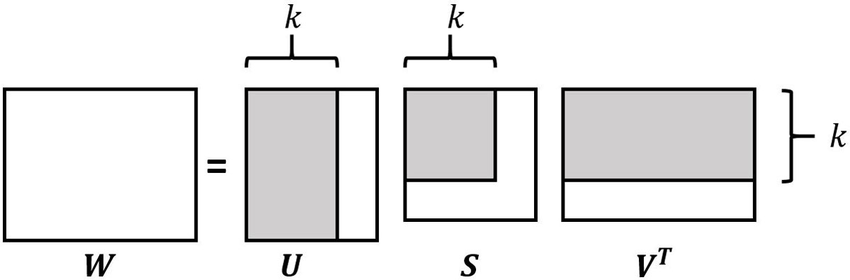
\includegraphics[width=0.8\linewidth]{images/svd.png}
  \caption{Troncamento della SVD \cite{img:svd}.}
\end{figure}

Problemi:
\begin{itemize}
  \item Se vogliamo aggiungere nuove parole dobbiamo ricalcolare la fattorizzazione perché cambia la dimensione della matrice.
  \item La matrice è comunque molto sparsa perché la maggior parte della parole non co-occorre.
  \item Costo quadratico per il calcolo della fattorizzata.
\end{itemize}

Una soluzione allo sbilanciamento delle frequenze può essere quella di ignorare le stop words, oppure pesare la co-occorrenza in base
alla distanza delle parole nel documento.

\subsection{GloVe}
Sia $X$ la matrice di term-context. Indichiamo con $X_{ij}$ la frequenza di una parola $j$ che occorre nel contesto della parola $i$, e $X_i$
la frequenza di una qualsiasi parola di apparire nel contesto della parola $i$.

Definiamo la probabilità di co-occorrenza $P_{ij}$, ovvero la probabilità che la parola $j$ occorra nel contesto della parola $i$.
\begin{align*}
  P_{ij} = P(j | i) = \frac{X_{ij}}{X_i}, \qquad X_i = \sum_k X_{ik}
\end{align*}

...

valutiamo il rapporto $\frac{P_{ik}}{P_{jk}}$

GloVe costruisce una funzione F che permette di imparare la rappresentazione.
%
\begin{align*}
  F(w_i, w_j, \tilde{w}_k) = \frac{P_{ik}}{P_{jk}}
\end{align*}

Minimizziamo una funzione obiettivo $J$.
\begin{align*}
  J = \sum_{\mathclap{\substack{i = 1, k = 1}}}^V f(X_{ik}) (w_i^T \tilde{w_k} + b_i + \tilde{b}_k - \log(X_{ik}))^2
\end{align*}

\section{Predictive Models}
I modelli predittivi provano direttamente a predire una parola dai termini vicini.

Il modello più usato è il Word2Vec, una rete neurale poco profonda con un hidden layer che permette di ricostruire il contesto di una parola.
Il raw text viene usato come training set di un approccio di apprendimento supervisionato.

Gli esempi di training vengono generati da coppie (target, context) scorrendo una finestra di dimensione fissa su
tutta la collezione.

Sia gli input che gli output sono codificati usando la rappresentazione one-hot.

Dopo avere eseguito l'addestramento la matrice dei pesi $W$ conterrà i word embedding del vocabolario $V$.

Il word embedding della parola $V_i$ sarà rappresentato dal vettore di N elementi $W_i = (w_{(i, 1)}, w_{(i, 2)}, ..., w_{(i, N)})$.

Word2Vec può produrre il word embedding utilizzando due architetture:
\begin{itemize}
  \item  \textbf{CBOW}

        Predice la parola corrente (target word) dalle vicine (context word).

        Funziona bene con training set piccoli e rappresenta bene le parole rare.
  \item \textbf{Skip-gram}

        Predice le parole vicine (context word) dalla parola corrente (target word).

        Molto più veloce del modello Skip-gram nella fase di addestramento e ha un accuratezza leggermente migliore nelle parole frequenti.
\end{itemize}

Metodi di training:
\begin{itemize}
  \item Hierarchical Softmax
  \item Negative sampling
\end{itemize}

\pagebreak

Grazie alla rete neurale è possibile catturare dei pattern complessi oltre la similarità tra le parole.

Più il training set è grande ($>10\text{M}$ parole) più le performance saranno migliori.

I testi devono includere più parole diverse possibili.

\begin{figure}[ht]
  \centering
  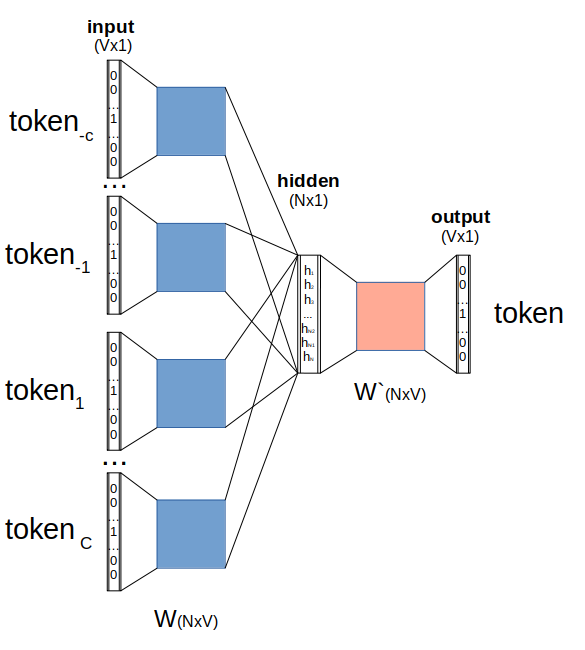
\includegraphics[width=0.5\linewidth]{images/cbow.png}
  \caption{Schema della rete con architettura CBOW \cite{wiki:CBOW}.}
\end{figure}

\begin{figure}[ht]
  \centering
  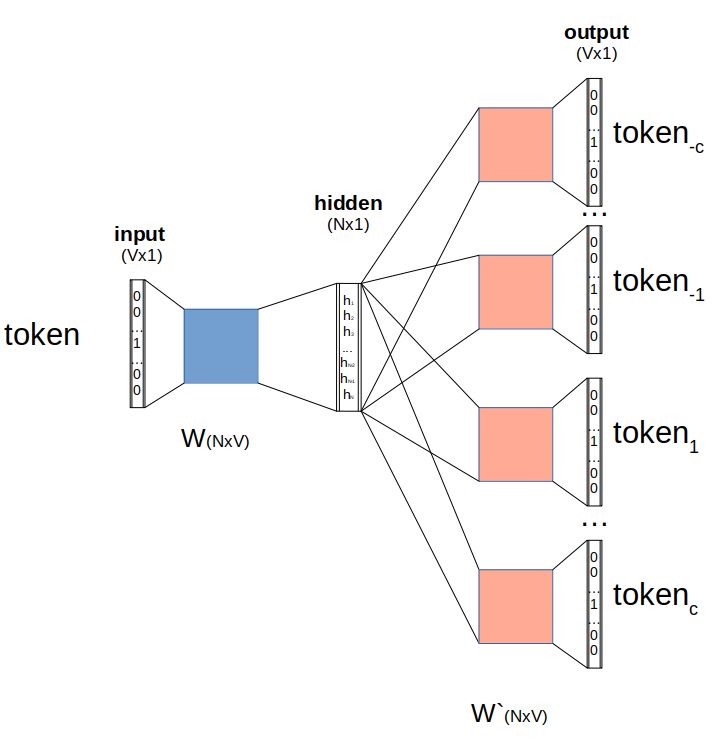
\includegraphics[width=0.55\linewidth]{images/skipgram.png}
  \caption{Schema della rete con architettura Skip-gram \cite{wiki:Skipgram}.}
\end{figure}
